\documentclass[10pt]{jarticle}
\usepackage{float}
\usepackage{adrobo_abst}
\usepackage[dvipdfmx]{graphicx}
\usepackage{amssymb,amsmath}
\usepackage{bm}
\usepackage[superscript]{cite}
\usepackage{enumerate}
\usepackage{url}
%\usepackage[absolute]{textpos}

\renewcommand\citeform[1]{(#1)}

\begin{document}
    
    \makeatletter
    \doctype{2021年度卒業論文概要}
  \title{      視覚と行動のend-to-end学習により経路追従行動を      オンラインで模倣する手法の提案}
        {(目標方向による経路選択機能の追加)}
    \etitle{A proposal for an online imitation method of path-tracking behavior   
    by end-to-end learning of vision and action}{(Addition of path selection function by target direction.)}
    
    \author{18C1096\hspace{.5zw}春山健太}
    \eauthor{Kenta HARUYMA}
    
    \makeatother
    
    % \abstract{We have proposed a method for acquiring autonomous driving by end-to-end learning using camera images and target directions, which can select a specific path depending on the target direction.
    % The effectiveness of the proposed method was verified by experiments using a simulator.
    \abstract{Previous research has shown that a robot can circumnavigate a certain path by end-to-end learning using camera images as input.
    We will Add the target direction to the dataset from the previous research and addition of path selection function for branching paths.
    We propose a method to acquire autonomous running by end-to-end learning with camera images and target direction as input, which can select a path according to the target direction.
    The proposed method was described in two phases: learning phase and testing phase.
    The effectiveness of the proposed method was verified by simulator experiments using a turtlebot3 waffle and crossroad environment.  
    % カメラ画像と目標方向を用いたend-to-end学習を用いた走行において,目標方向によって特定の経路を選択する手法を提案した.実験により提案手法の有効性を検証した.
    }
    \keywords{end-to-end Learning, Navigation, Target Direction}
    
    \maketitle
    
    \supervisor{指導教員:林原靖男 教授}
    
    \section{緒\hspace{2zw}言}%===========================
    近年,カメラ画像に基づいた自律移動の研究が行われている.%\cite{nvidia}.
    Bojaskiら\cite{nvidia}は,人間のハンドル操作によるステアリング
    角度の模倣学習を行い,画像を用いて走行する手法を提案している.
    また岡田ら\cite{okada}は,
    LiDARとオドメトリのデータを入力とする
    ルールべースの制御器による経路追従行動を,
    カメラ画像によるend-to-end学習によって
    模倣する手法を提案している.
    % その制御器の出力する角速度とロボットに取り付けたカメラから取得したカメラ画像を用いて
    % 学習器の訓練を行い,学習後はカメラ画像のみを用いて自律移動を行う.
    % ルールベースの制御器を用いることでデータセットを自動的に収集し,
    % その経路追従行動を模倣する手法を提案している.
    上記の研究により,カメラ画像を用いて,
    ロボットが一定の経路を周回することが可能であると示されている.
    本研究では,岡田らの研究をベースに,\reffig{bunki}のような分岐路において,
    「直進」と「左折」などの経路選択する機能を追加することを検討する.
    また構築したシステムを用いた実験を行い,機能の有効性を検証する.
    % カメラ画像のみでは,「どちらへ進むか」のような経路選択に必要な情報が不足している可能性がある.
    % 具体的には,データセットへ,従来のカメラ画像以外に「直進」「左折」などの
    % 目標とする進行方向の情報(本研究では”目標方向”とする )を追加する
    % ことで,経路の選択を行える可能性がある.

    % 本研究では目標方向によって経路の選択が可能な,
    % カメラ画像と目標方向を入力したend-to-end学習による自律走行を
    % 獲得する手法を提案する.
    % また提案手法に基づいて,構築したシステムを用いた実験を行い,
    % 提案手法の有効性を検証する.
    \begin{center}
        \begin{figure}[h]
            \centering
            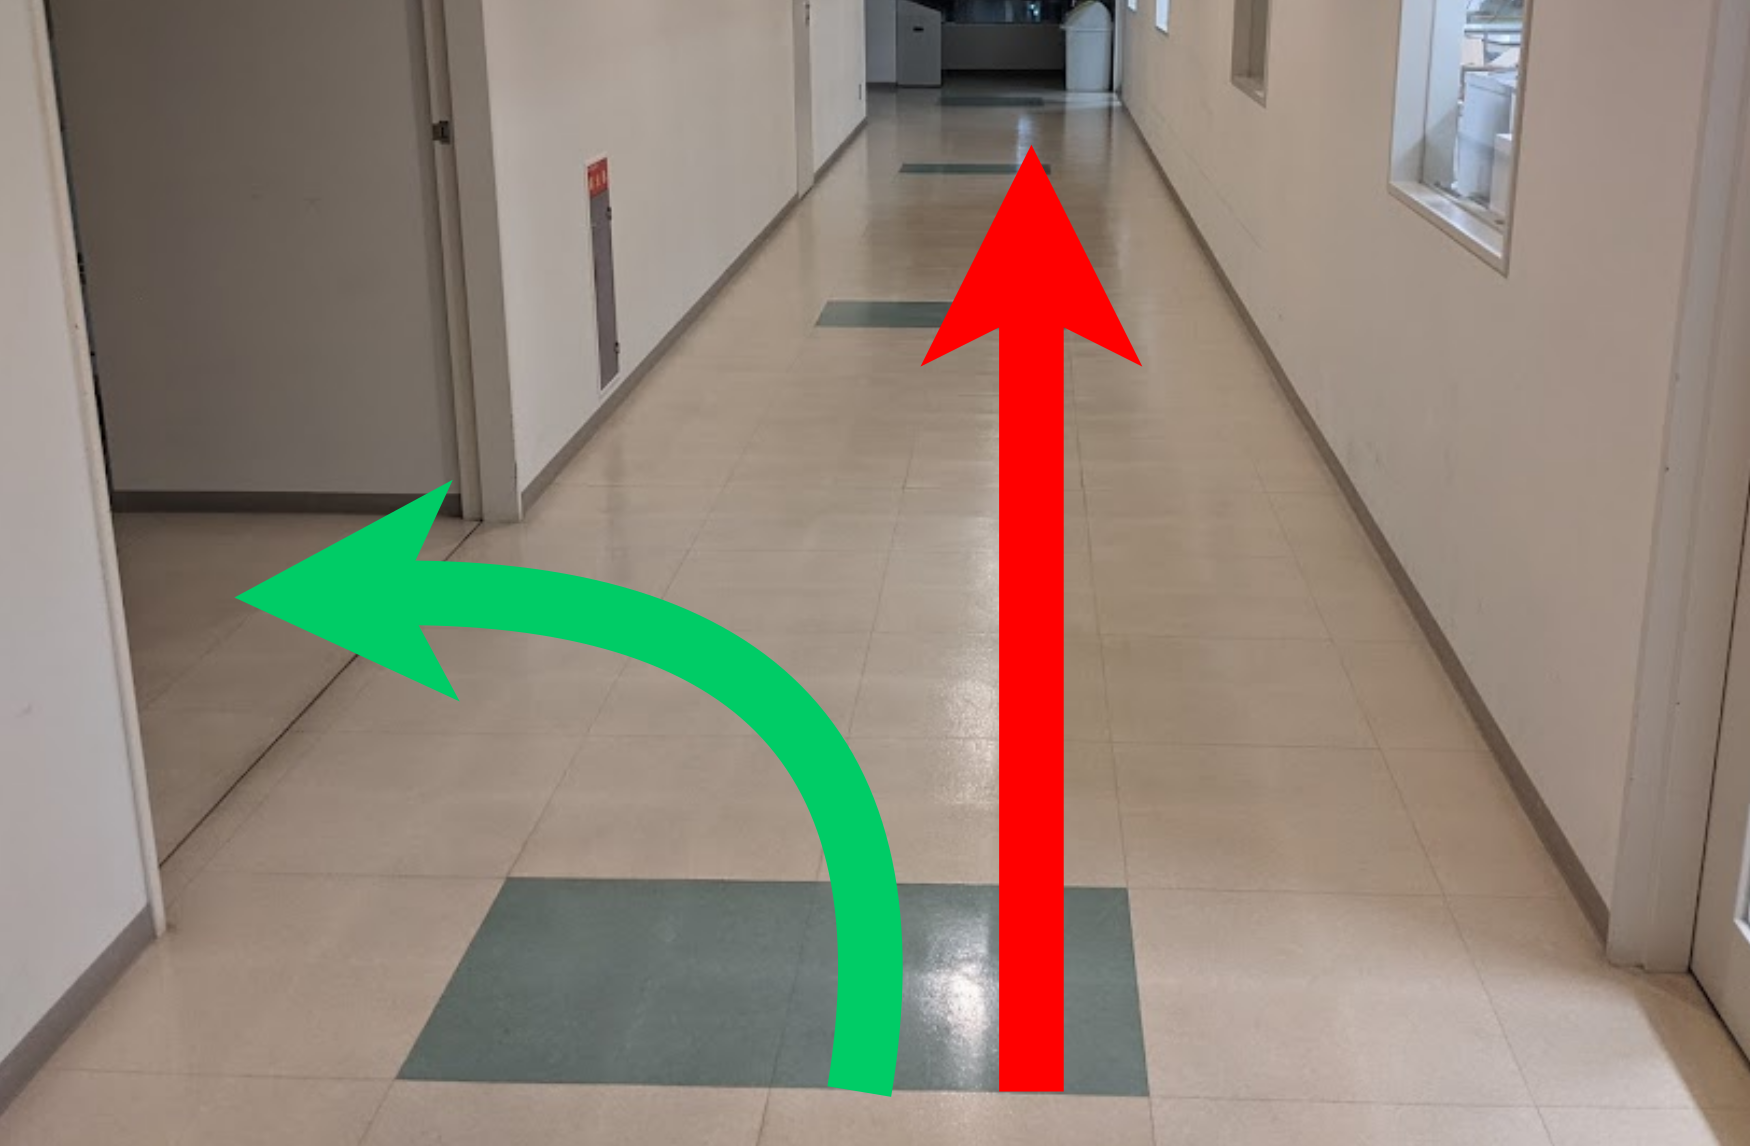
\includegraphics[width=5cm]{./fig/zyuzibunki.png}
            \caption{Path selection}
            \label{fig:bunki}
        \end{figure}
    \end{center}
    \section{提案手法}%===========================
    % \begin{figure}[h]
    %     \begin{tabular}{c}
    %       \begin{minipage}[t]{0.5\hsize}
           
    %         % \vspace{-1.0zh}
    %         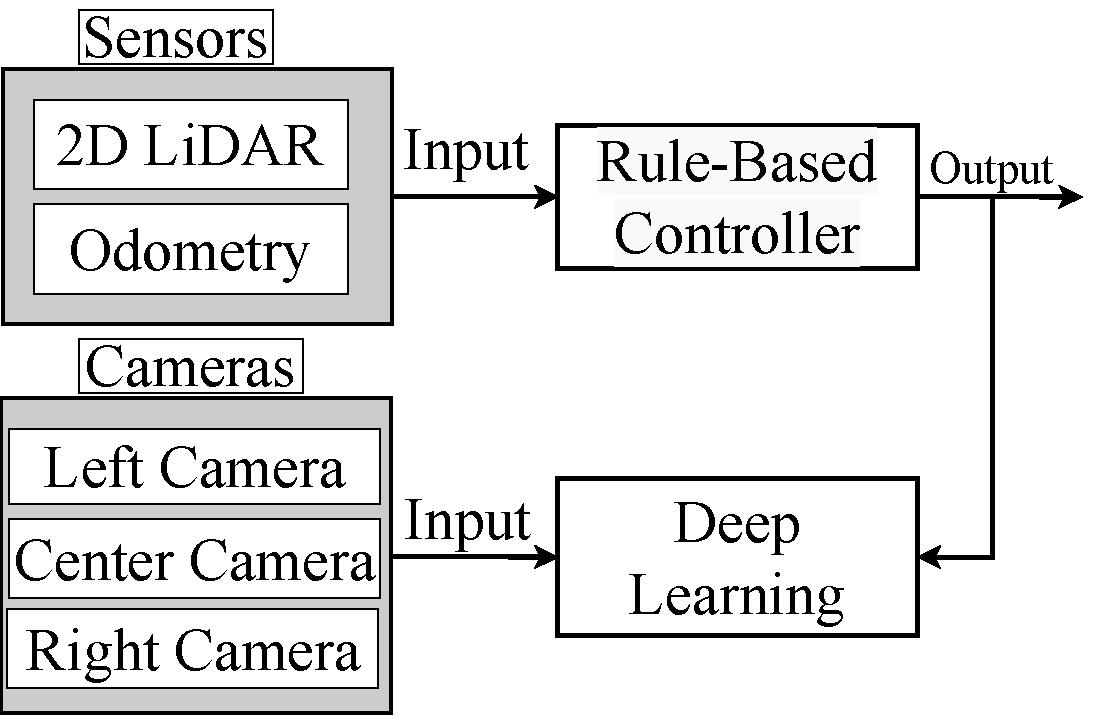
\includegraphics[width=5cm]{./fig/learning_okada.pdf}
    %         % \subcaption{Learning phase}
    %         \label{fig::learning_abs}
    %       \end{minipage}
    %       \begin{minipage}[t]{0.5\hsize}
    %       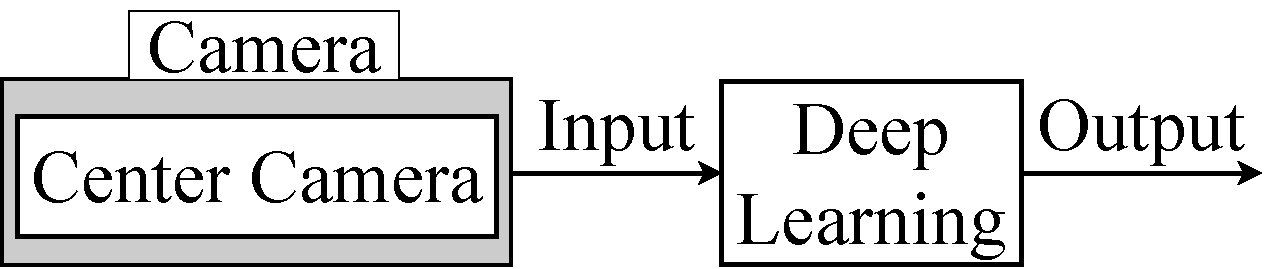
\includegraphics[width=5cm]{./fig/test_okada.pdf}
    %         % \subcaption{Test phase}
    %         \label{fig::test_abs}
    %       \end{minipage}
    %     \end{tabular}
    %      \caption{Concept of the proposed method}
    %      \label{fig::method_abs}
    % \end{figure}
    はじめに,経路選択をする機能
    「直進」「左折」などの目標とする進行方向の情報(本研究では”目標方向”とする )を追加する
    本研究で用いた目標方向とデータ形式を,\reftab{data}に示す.
    分岐路以外での「道なり」を示す(continue)
    分岐路を「直進(go straight)」「左折(turn left)」
    「右折(turn right)」の4つとする.
    \begin{table}[h]
        \caption{Target direction and data}
        \label{tab:data}
        \begin{center}
            \vskip 0.5zh
            \begin{tabular}{|c|c|}
                \hline
                Target direction & Data\\ \hline
                continue & $[100, 0, 0, 0]$ \\ \hline
                go straight & $[0, 100, 0, 0]$ \\ \hline
                turn left& $[0, 0, 100, 0]$ \\ \hline
                turn right & $[0, 0, 0, 100]$ \\ \hline
            \end{tabular}
        \end{center}
    \end{table}
    % 目標方向によって経路の選択が可能な,
    % カメラ画像と目標方向を入力したend-to-end学習による自律走行の獲得
    % を目的として,
    次に本研究のベースとする岡田らの\cite{okada}と,提案手法を併せて述べる.

    % \begin{center}
    %     \begin{figure}[h]
    %         \centering
    %         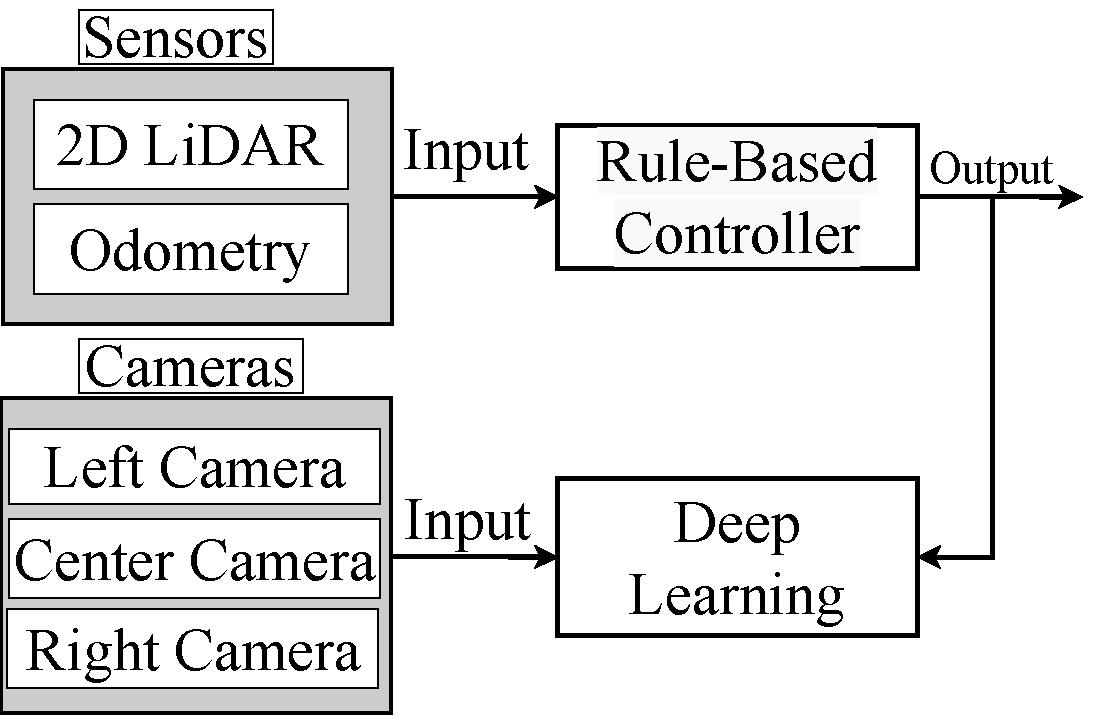
\includegraphics[width=6cm]{./fig/learning_okada.pdf}
    %         \caption{Learning phase}
    %         \label{fig:learning_okada}
    %     \end{figure}
    % \end{center}
    % \begin{center}
    %     \begin{figure}[h]
    %         \centering
    %         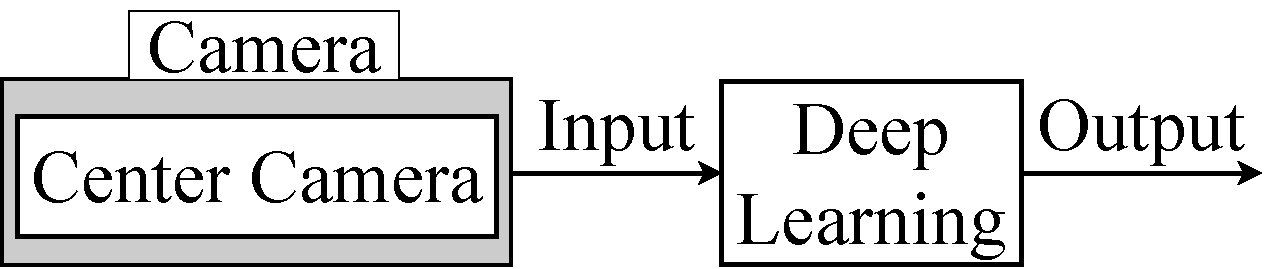
\includegraphics[width=6cm]{./fig/test_okada.pdf}
    %         \caption{Learning phase}
    %         \label{fig:test_okada}
    %     \end{figure}
    % \end{center}
    まずはじめに,学習器の訓練を行う「学習フェーズ」を述べる
    % 走行における並進速度は2つのフェーズで固定した同じ値を用いる.
    %=======================
    % \subsection{学習フェーズ}
    学習フェーズで用いるシステムを\reffig{system_learning}に示す.
    岡田らの研究では,
    LiDARとオドメトリを入力とする地図ベースの制御器による経路追従行動を,
    カメラ画像を用いてend-to-endで模倣学習する.
    提案手法では,地図ベースの制御器へ目標方向の生成機能を加え,
    学習に用いるデータセットへ目標方向を追加する.
    % ROS Navigation\_stack\cite{navigation}であり,LiDARとオドメトリを入力とするルールベースの制御器である.
    学習器の訓練は,「訓練データ(カメラ画像,目標方向)を学習器へ入力し,結果を出力(角速度)」を1stepとして,
    設定したstep数行う.
    また走行に用いる並進速度は固定した値を用いる.
    % 1)LiDARとオドメトリから得たデータを入力とする地図ベースの制御器の出力を用いて自律走行する.
    % 2)地図ベースの制御器の出力からヨー方向の角速度と目標方向,ロボットに取り付けた3つのカメラから
    % RGB画像を取得し,訓練データへ加える.
    % 3)訓練データ(入力:カメラ画像,目標方向 目標出力:角速度)を用いてend-to-end学習を行い,学習器の出力を記録.
    % \begin{enumerate}
    %     \setlength{\parskip}{0cm} % 段落間
    %     \setlength{\itemsep}{0cm} % 項目間
    %     \item LiDARとオドメトリから得たデータを入力とする地図ベースの制御器の出力を用いて自律走行する
    %     \item 地図ベースの制御器の出力からヨー方向の角速度と目標方向,ロボットに取り付けた3つのカメラから
    %     RGB画像を取得し,訓練データへ加える.
    %     \item 訓練データ(入力:カメラ画像,目標方向 目標出力:角速度)を用いてend-to-end学習を行い,学習器の出力を記録
    %     \end{enumerate}
    \begin{center}
        \begin{figure}[h]
            \centering
            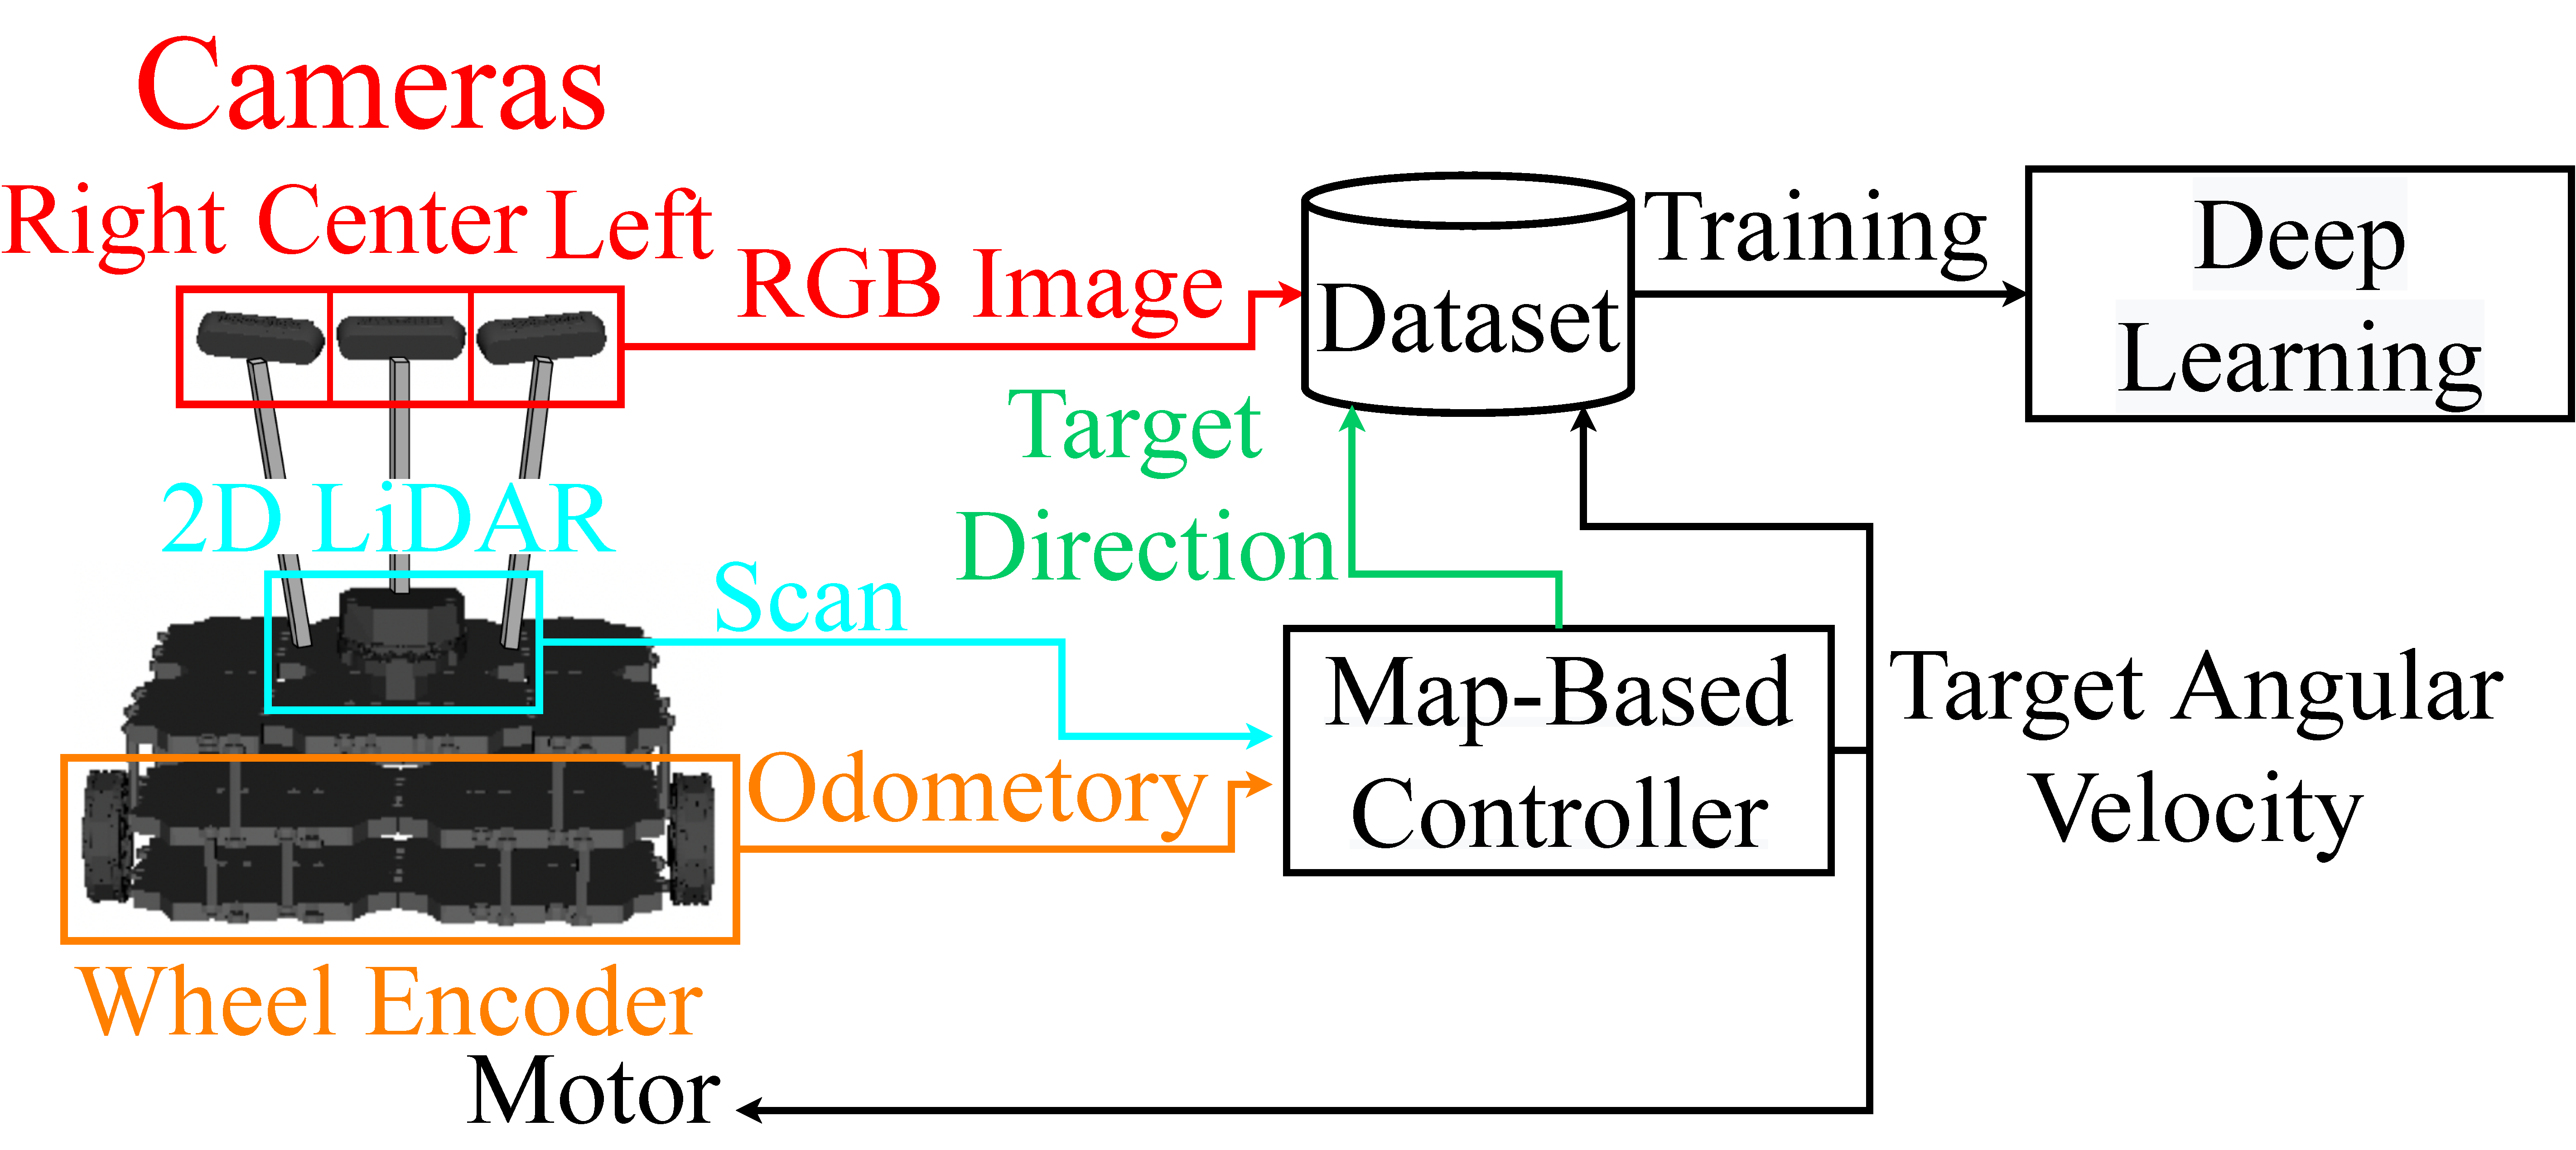
\includegraphics[width=0.46\textwidth]{./fig/system_learning.pdf}
            \caption{Learning phase}
            \label{fig:system_learning}
        \end{figure}
    \end{center}
    %=========================
    % \subsection{テストフェーズ}

    設定したstep数に達した場合,
    \reffig{system_test}で示す,
    訓練した学習器の出力を用いて走行する「テストフェーズ」へ移行する.
    % テストフェーズでの目標方向は,Joystickコントローラのボタンを用いて入力する.
    岡田らの研究では,カメラ画像を学習器へ入力し,
    学習器の出力(角速度)を用いて自律走行する.
    提案手法では,入力へ目標方向を追加した学習器の出力を用いる.
    % \begin{enumerate}
    % \setlength{\parskip}{0cm} % 段落間
    % \setlength{\itemsep}{0cm} % 項目間
    % \item ロボット中央のカメラからRGB画像 ,Joystickコントローラより目標方向のデータを取得.
    % \item 取得したデータ (カメラ画像,目標方向)を学習器へ入力.
    % \item 固定した並進速度,学習器の出力(角速度)を用いて走行.
    % \end{enumerate}
    \begin{center}
        \begin{figure}[h]
            \centering
            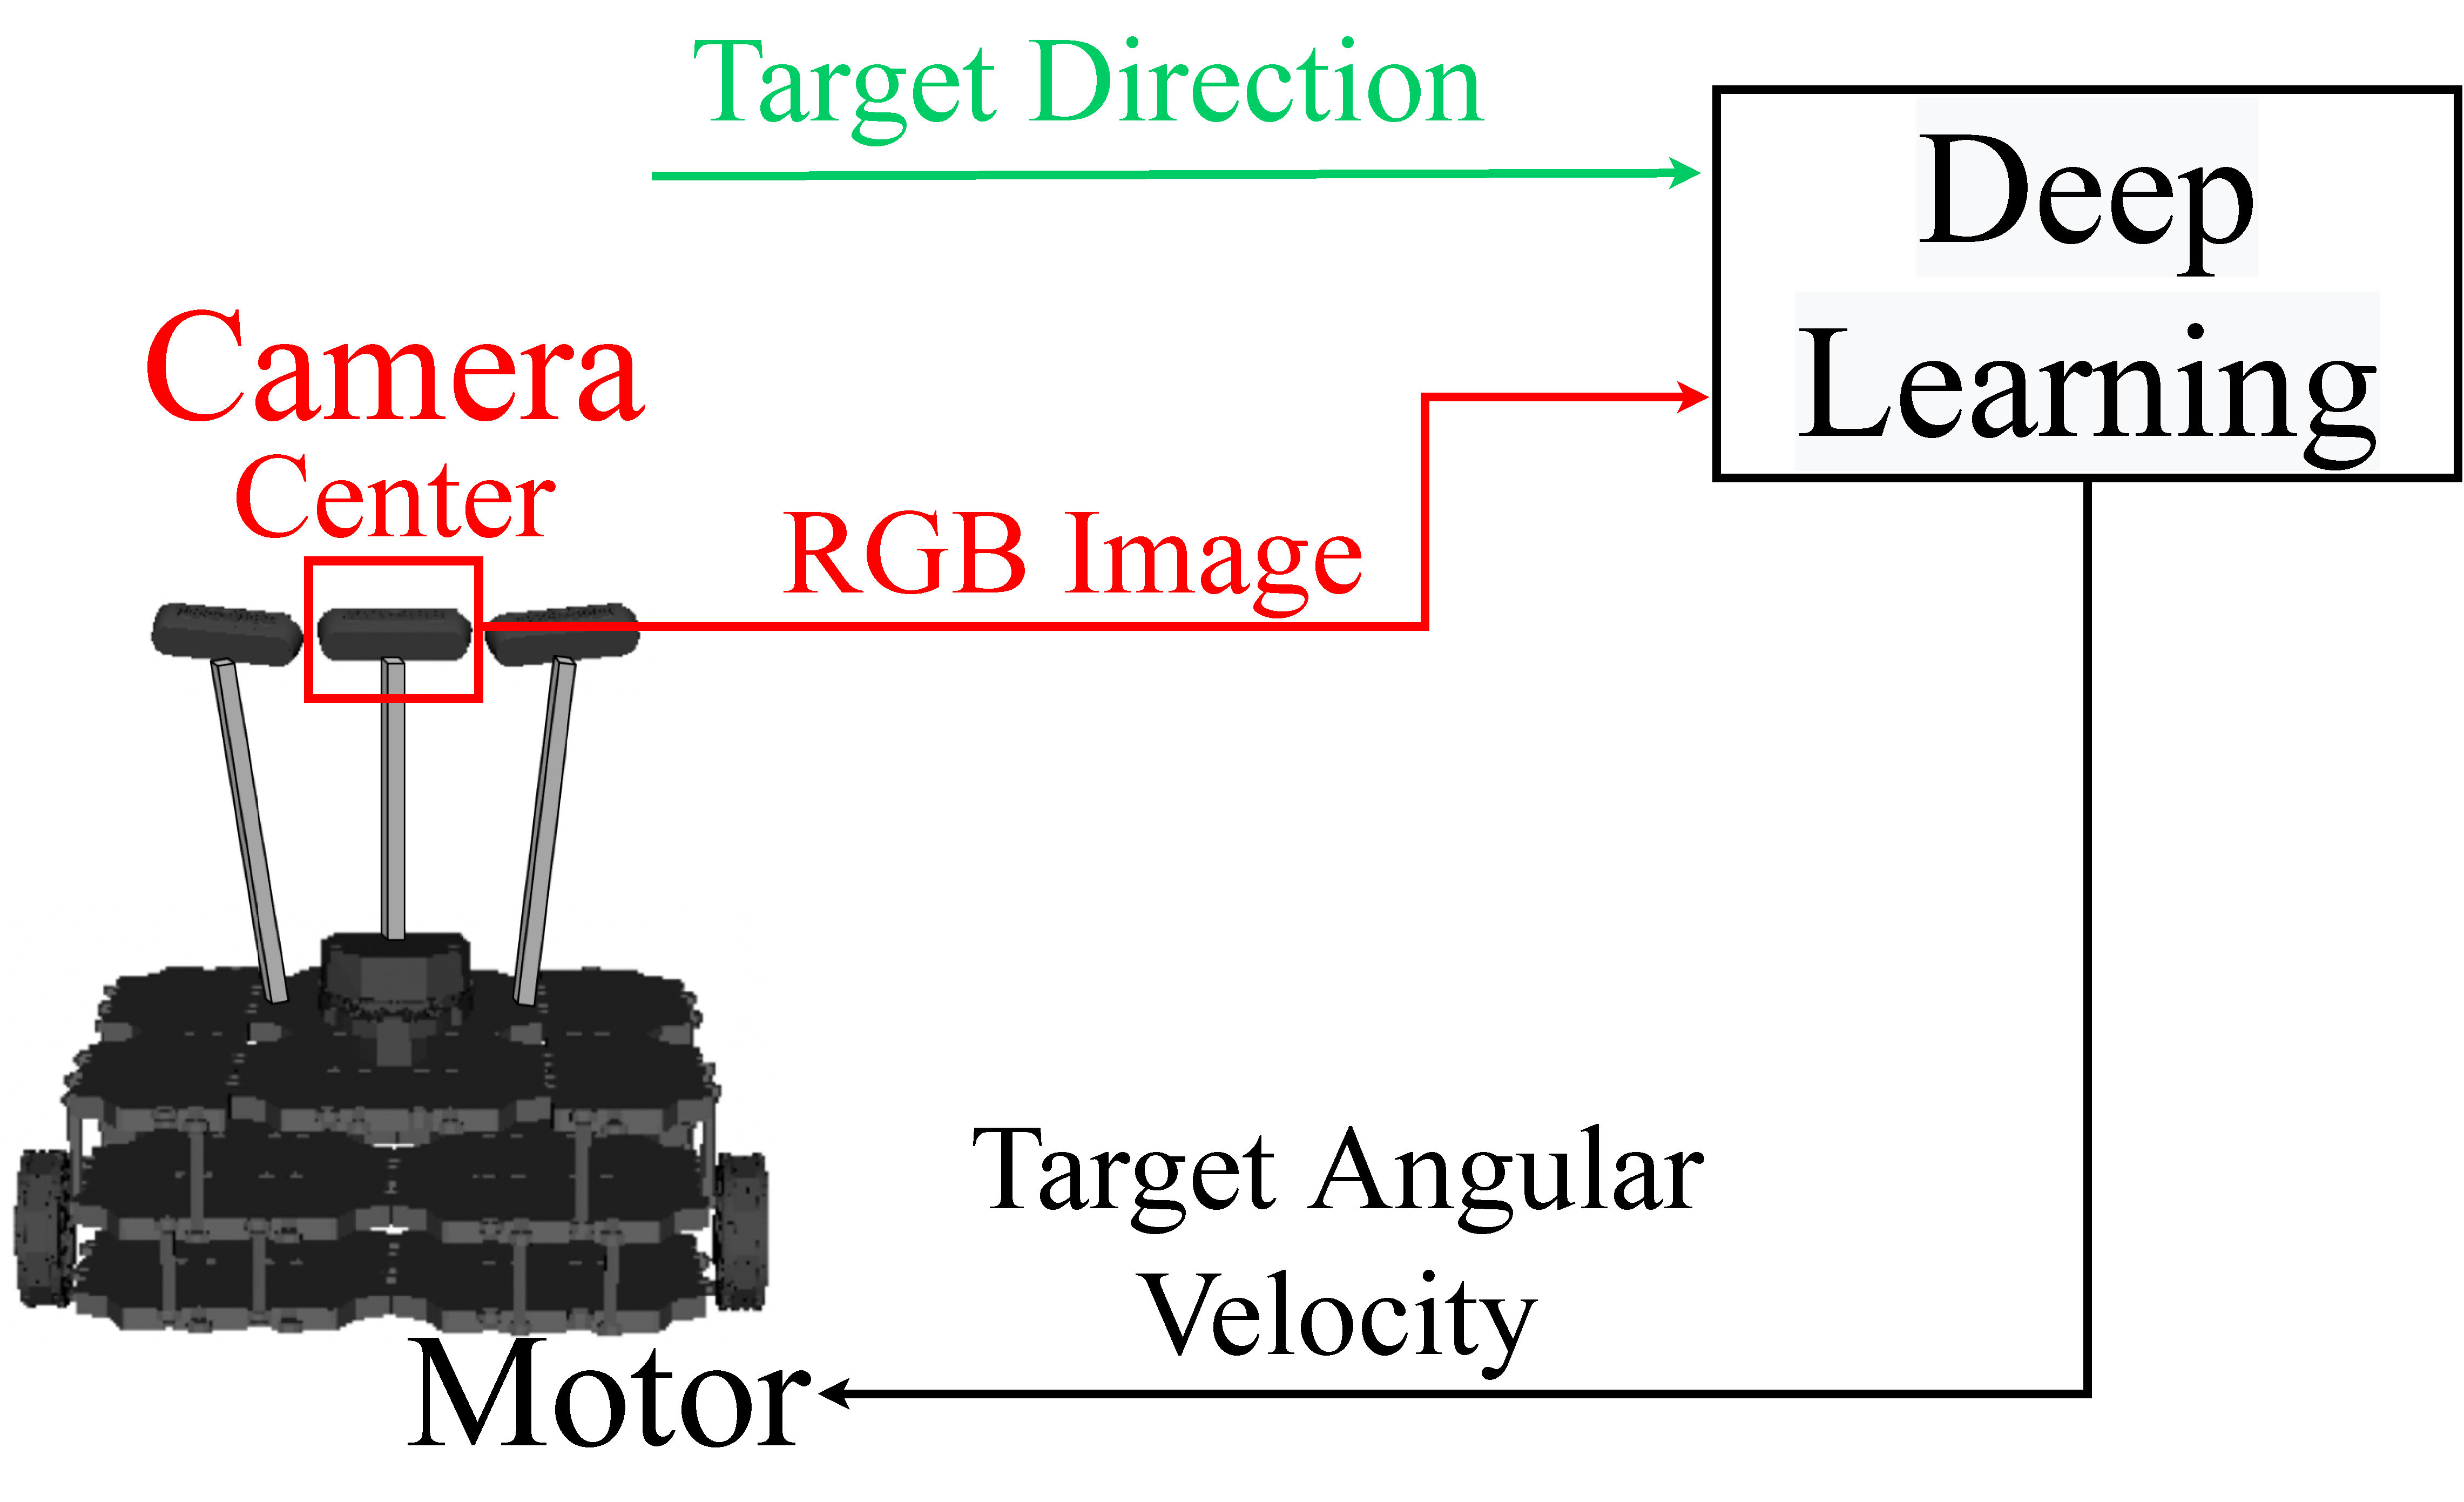
\includegraphics[width=6.1cm]{./fig/system_test.pdf}
            \caption{Test phase}
            \label{fig:system_test}
        \end{figure}
    \end{center}
    \vspace{-1zh}
    \section{実\hspace{2zw}験}%=========================検証
    提案手法の有効性の検証のため,
    3DロボットシミュレータGazebo上で実験を行う.
    実験装置として\reffig{system_learning},\reffig{system_test}で示した
    Turtlebot3 waffleへカメラを3つ追加したモデルを用いる.
    \reffig{exp}に用いた環境,経路と入力する目標方向を示す.
    環境は道幅が2.5[m]の十字路を用いる.
    % 実験は下記の手順で,経路をStart-Aを固定し,目標地点をB,C,Dと変更して
    学習フェーズではstep数を6000[step],訓練フェーズでは各経路を10回走行する.
    並進速度は0.2[m/s]とした.
    \begin{enumerate}
        \setlength{\parskip}{0cm} % 段落間
        \setlength{\itemsep}{0cm} % 項目間
        \item Start - A - Target point(B)
        \item Start - A - Target point(C)
        \item Start - A - Target point(D)
        \end{enumerate}
    実験条件は,
    テストフェーズにおいて「壁に衝突せず,指定した目標地点へ到達」を成功
    「目標方向とは異なった経路を選択,または壁に衝突」を失敗とする.
    \begin{center}
        \begin{figure}[h]
            \centering
            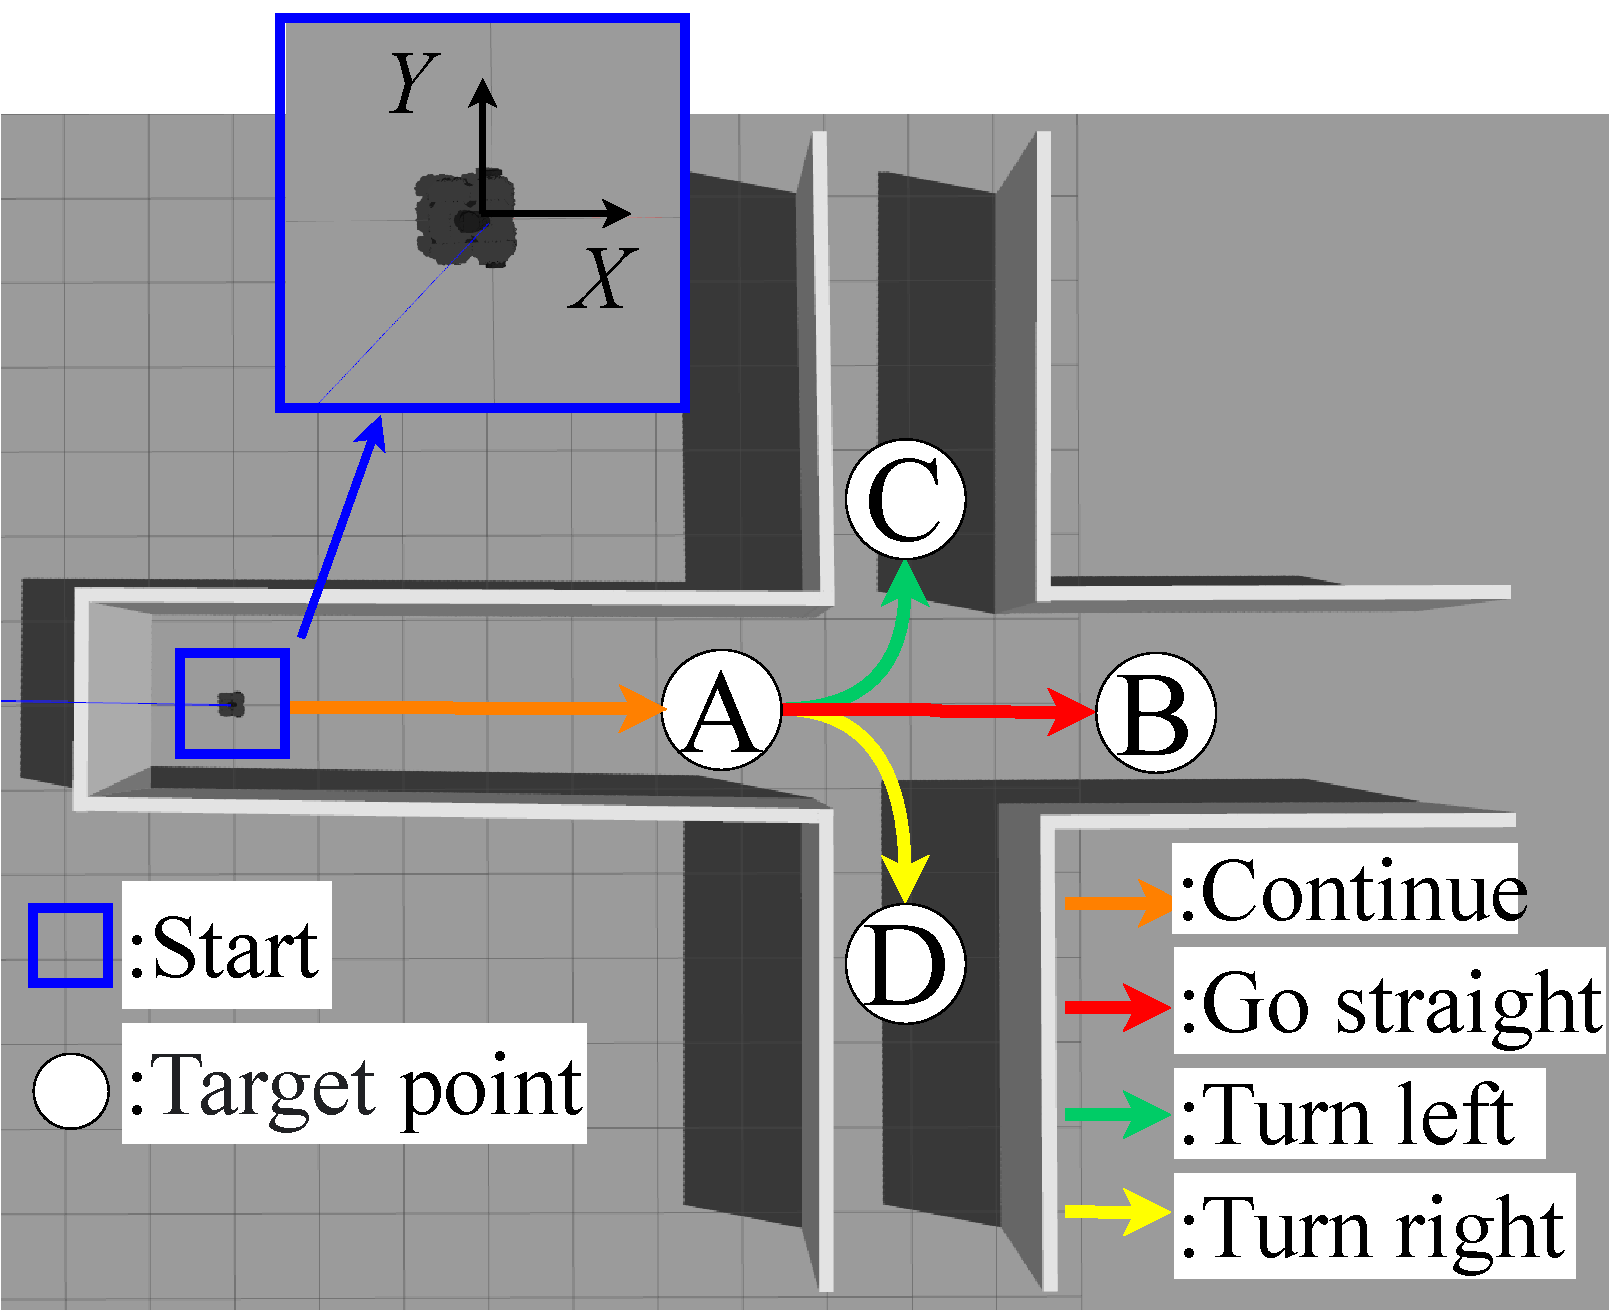
\includegraphics[width = 6.7cm]{./fig/zyuziroute.pdf}
            
            \caption{Environment and route for experiment}
            \vskip 0.1zh
            \label{fig:exp}
        \end{figure}
    \end{center}
    % \begin{enumerate}
    %     \setlength{\parskip}{0cm} % 段落間
    %     \setlength{\itemsep}{0cm} % 項目間
    %     \item 学習フェーズによって,学習器の訓練 ( 経路の学習 ) 行う
    %     ( 制御:地図べースの制御器の出力 )
    %     \item 設定した step 数を学習後,訓練フェーズへ移行
    %     ( 制御:学習器の出力 )
    %     \item コース内に設定した地点において目標方向のコマンドを入力,挙動を確認
    % \end{enumerate}
   \section{実験結果}
   実験結果を\reftab{suc}に示す.
   結果から,目標方向によって経路を選択する提案手法の有効性が確認できた.
   \begin{table}[H]
    \caption{Number of successes experiment}
    \label{tab:suc}
    \begin{center}
        \vskip -1zh
        \begin{tabular}{|c|c|}
            \hline
            Route and Target direction & Number of successes\\ \hline
            % Start - A (continue) & $10/10$ \\ \hline
            Start - A - B (go straight) & $10/10$ \\ \hline
            Start - A - C (turn left) & $10/10$ \\ \hline
            Start - A - D (turn right) & $10/10$ \\ \hline
        \end{tabular}
    \end{center}
\end{table}
    \section{結\hspace{2zw}言}%===========================
    本稿では,目標方向によって経路を選択可能な,
    カメラ画像と目標方向を入力とするend-to-end学習による自律走行を
    獲得する手法を提案した.
    またシミュレータを用いた実験により,提案手法の有効性を検証した.
    
    {\footnotesize
        \begin{thebibliography}{99}
            
            % \bibitem{工大2005}
            % 工大太郎: ``ロボットのしくみ'', 
            % 日本機械学会論文誌A, 
            % Vol.~108, No.~1034 (2005), pp.~1--2.
            
            \bibitem{nvidia}
            Mariusz Bojarski et al:``End to End Learning for Self-Driving Cars'',
            arXiv: 1604.07316,(2016)
            \bibitem{okada}
            岡田眞也, 清岡優祐, 上田隆一, 林原靖男:``視覚と行動の end-to-end 
            学習により経路追従行動をオンラインで模倣する手法の提案''
            SICE-SI2020予稿集,1147--1152,制御学会SI部門講演会(2020)
            \bibitem{navigation}
            ros-planning,navigation:
            \url{https://github.com/ros-planning/navigation}, 
            (参照日 2020年12月30日). 
            % \bibitem{Shibutani2004}
            % Y. Shibutani: ``Heinrich's Law Resulted Pattern Dynamics --Part2--'',
            % Proceedings of the 79th Kansai Branch Regular Meeting of the Japan Society of Mechanical Engineers,  
            % No.~04--05 (2004), pp.~205--206.
            
            % \bibitem{Handbook1979}
            % The Japan Society of Mechanical Engineers ed.: ``JSME Date Handbook: Heat Transfer'', 
            % (1979), p.~123, The Japan Society of Mechanical Engineers.
            
            % \bibitem{Kikuchi2017}
            % K. Kikuchi, M. Miura, K. Shibata, J. Yamamura: ``Soft Landing Condition for Stair-climbing Robot with Hopping Mechanism'', 
            % Journal of JSDE, Vol.~53, No.~8 (2018), pp.~605--614, \url{https://doi.org/10.14953/jjsde.2017.2774}.
        \end{thebibliography}
    }
   
        
   
    \vspace{5truemm}
    
    \normalsize
    
\end{document}
